Метод SHAP несколько отличается от использования значений Шэпли напрямую для интерпретации вклада признаков -- он модифицирует классический подход. Рассмотрим SHAP подробнее.

Вместо использования большого количества моделей мы обучим одну модель и далее будем пользоваться только ее предсказаниями. Тогда наша модель представима в виде $f: \re^d \rightarrow \re$. Вместо исключения из нее признаков (в таком случае нам пришлось бы переобучать модель) мы оставим данные признаки в виде случайных величин и посчитаем математическое ожидание предсказания при фиксированных включенных в модель признаках \cite{basis, shap}.

Для упрощения расчетов мы не будем рассматривать разные значения предикторов, а бинаризуем их представление, обозначив за <<1>> наличие предиктора и за <<0>> его отсутствие: $x \rightarrow x', \, x' = \{1\}^d$. % не знаю корректно ли
Обозначим за $z' \in \{0,1\}^d$ объект, у которого мы учитываем только признаки из $S$ при формировании предсказания:
$z_j =
\begin{cases}
1, \text{если $j \in S$}\\
0, \text{если $j \notin S$}\\
\end{cases}$.\\
То есть $z'$ -- одна из возможных комбинаций предикторов \cite{basis, shap}.

Обученная модель работает с исходным видом признаков, поэтому нам нужно также восстанавливать значения исходных признаков по бинарному вектору. Введем для этого функцию $h_x(z') = z$, где $x$ -- исходный вектор исследуемого объекта, $z'$ -- бинарный вектор, в котором некоторые признаки заменены нулями, $z$ -- представление вектора $z'$ в исходном пространстве признаков \cite{basis}.

\vspace{-3mm}
\begin{figure}[h]
	\centering{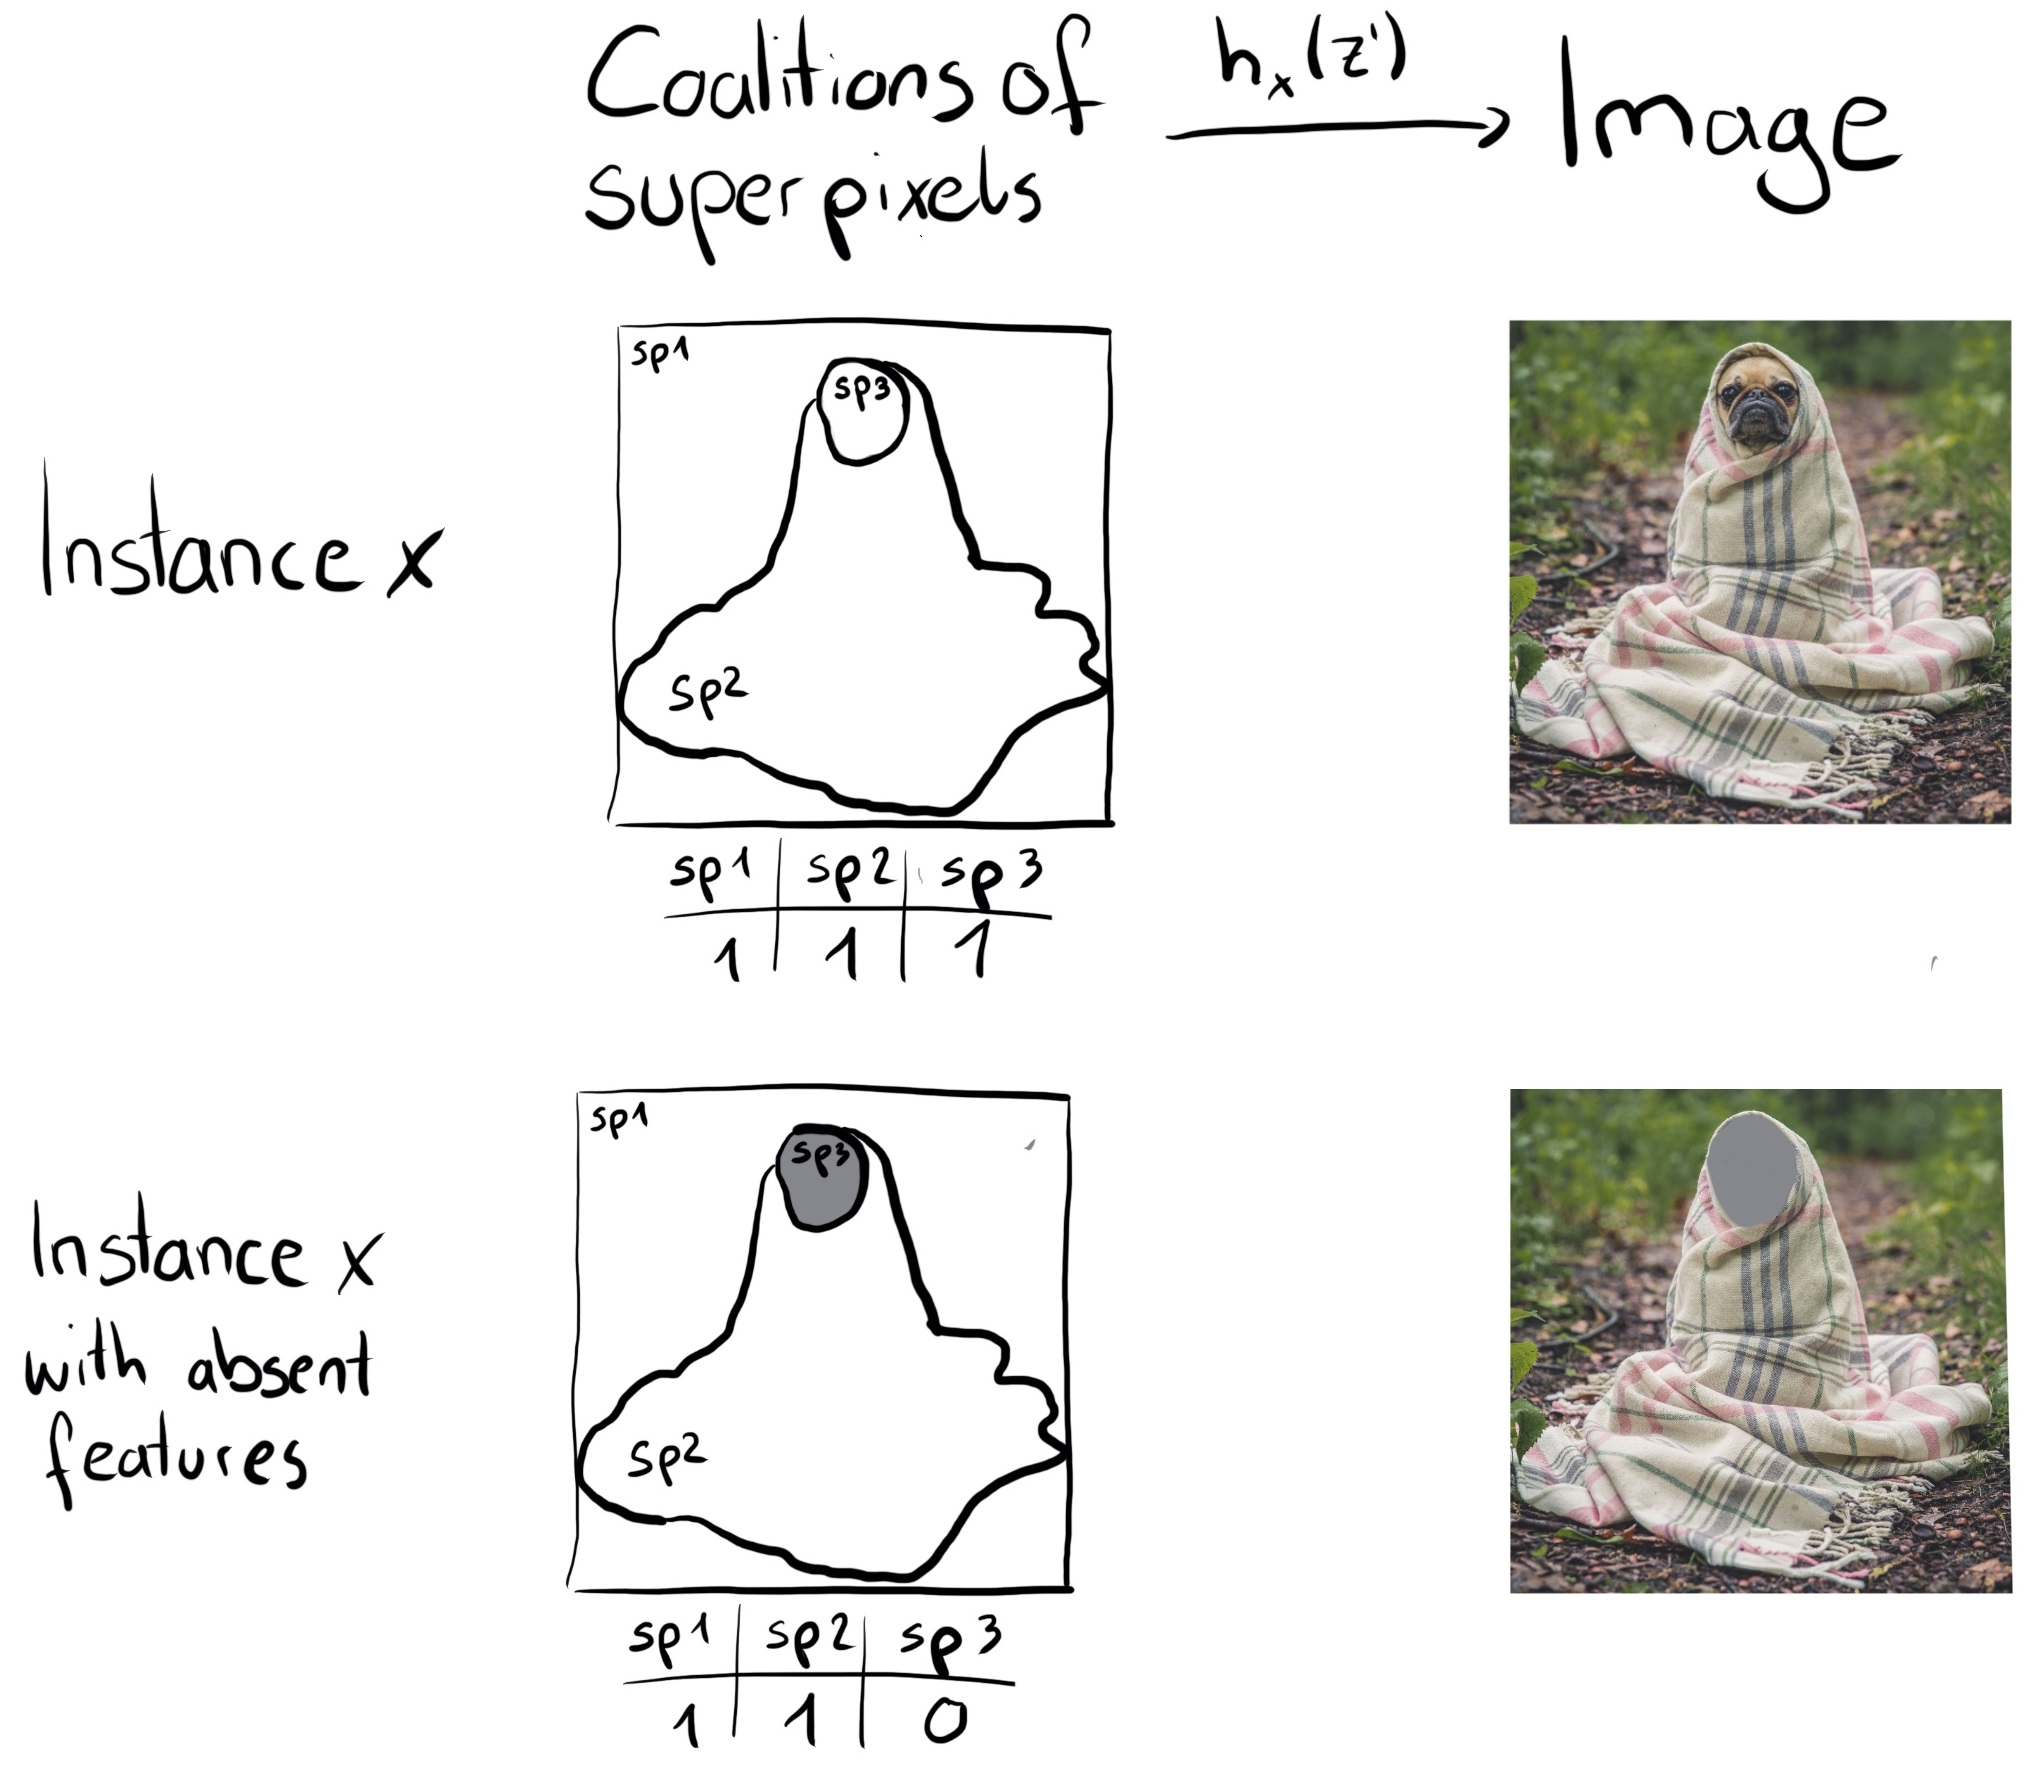
\includegraphics[width=0.6\linewidth]{pics/shap3.png}}
\end{figure}
\vspace{-3mm}

Функция $h_x$ вместо единиц восстанавливает значения из вектора $x$, а вместо нулей оставляет признак как некоторую переменную (случайную величину).
% наверняка можно как-то умнее упрощать признаки
Тогда наше ожидаемое предсказание для $z$ представимо в виде математического ожидания:
\[
\bar{f}(z) = \e(f(z)|\,z_S)
\]

Мы знаем конкретные значения признаков $z_S$, так как функция $h_x$ перенесла их из объекта $x$. Найдя математическое ожидание мы можем подставить данные значения, чтобы получить условное математическое ожидание, которое и будет оценкой нашего предсказания. Данную формулу мы можем использовать при расчете необходимых значений \cite{basis}.% здесь для его расчета мы почему-то переходили к безусловному матожиданию, это связано со свойствами значений Шэпли -- не уверена нужно ли это прописывать

Поскольку мы не знаем истинное распределение, чтобы иметь возможность посчитать матожидание, аппроксимируем его оценкой. Для этого немного изменим функцию $h_x$ -- теперь вместо нулей она будет проставлять случайные значения соответствующих признаков. Тогда для каждого множества $S$ мы сможем получить несколько предсказаний модели и усреднить их \cite{basis}:
\[
\hat{f}(z) = \frac{1}{k} \sum\limits_{i=1}^k f(z_{F\backslash S}, z_S),
\]
где $z_{F\backslash S}$ -- исключенные из модели признаки, вместо которые подставлены случайные значения, $z_S$ -- включенные в модель признаки, значения которых известны из исследуемого объекта $x$.
\vspace{-2mm}

\paragraph{Kernel SHAP.}% я очень хочу доказать то, что они доказали
Авторы алгоритма показали, что есть упрощенный способ найти значения Шэпли: % с оговоркой про то что это не значения Шэпли
с помощью взвешенного МНК. В нем аналогично перебираются разные комбинации $z'$ -- так формируется выборка $Z$ для регрессии. Зависимой переменной является предсказание модели для сгенерированной выборки (переведенной в исходное пространство признкаов): $y_i = f(h_x(z'_i)) = f(z_i)$, где $z'_i$ -- строка матрицы $Z$. Тогда решением нашей задачи является вектор \cite{basis}: \[
\phi = (Z^T W Z)^{-1} Z^T W y
\]
\vspace{-6mm}
% нужно ли говорить про корреляцию признаков. они это указывают как раз при расчете условного матожидания, и здесь наверное аналогия в мультиколлинеарности, но это неточно

Чтобы коэффициенты в регрессии соответствовали искомым значения, веса должны быть заданы диагональной матрицей $W$ \cite{shap}: 
\[w_{ii}(z'_i) = \frac{|F|-1}{
	\begin{pmatrix}
	|F| \\
	|S_i|
	\end{pmatrix} \cdot |S_i| \cdot (|F| - |S_i|)} = \frac{|F|-1}{|F|} \cdot \frac{|S_i - 1|! \cdot (|F|-|S_i|-1)!}{(|F|-1)!},
\]
где $|S_i|$ -- количество элементов в множестве $S_i$, то есть количество ненулевых элементов в $z'_i$.

В данном случае коэффициент при константе будет показывать предсказание модели при отсутствии признаков. Коэффициенты при признаках являются соответствующими значениями Шэпли, % если так можно сказать. мб сноска
которые можно использовать для интерпретации их вклада в предсказание \cite{basis}.

Ранее мы уже говорили о том, что комбинации, в которых либо почти все нули, либо почти все единицы имеют больший вес при расчете значений Шэпли. Данный факт сохраняется и в линейной регрессии, поэтому формируя выборку можно отдавать предпочтение именно данным примерам -- в случае, если мы ограничены в количестве наблюдений \cite{basis}.

Интересно, что если записать задачу в более общем виде:
\[
\sum\limits_{z' \in Z} (f(h_x(z')) - g(z'))^2 \cdot \underbrace{\frac{|F|-1}{|F|} \cdot \frac{|S - 1|! \cdot (|F|-|S|-1)!}{(|F|-1)!}}_{w(z') = \pi_x(z')} = L(f, g, \pi_x) + \Omega(g) \rightarrow \min_g
\]
\vspace{-4mm}

мы получим ровно ту же задачу, что решает LIME. То есть при определенных гиперпараметрах LIME и SHAP эквивалентны друг другу \cite{shap}.
% регуляризация -- легально ли это, мы ведь хотим значения Шэпли хммм
% сказать что бесконечные веса -- я как-то устранила :О

Существуют и другие модификации SHAP: TreeSHAP, Linear SHAP, Low-Order SHAP, Max SHAP, Deep SHAP и др. В отличие от классического подхода они специфицированы для отдельных классов моделей, что позволяет снизить время работы алгоритма \cite{basis, shap}.